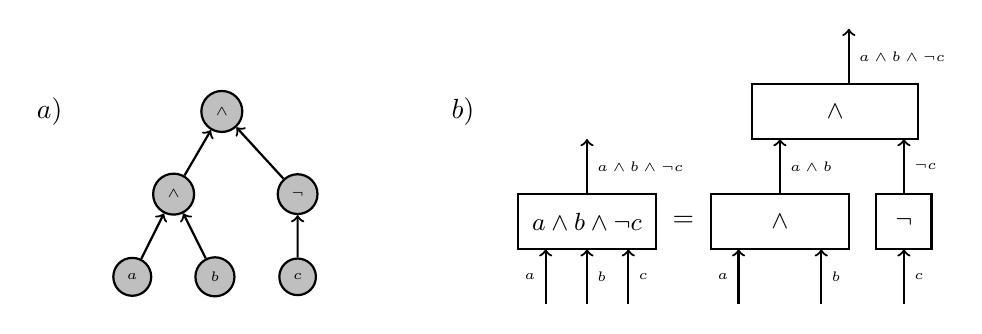
\begin{tikzpicture}[scale=0.35, yscale=-1, thick] % , baseline = -3.5pt

\begin{scope}[shift={(-15,0)}]

\node[anchor=center] (text) at (-3,-6) {${a)}$};

	\node [circle, draw, thick, fill=gray!50] (T1) at (0,0) {\tiny $\catvariableof{a}$};
	\node [circle, draw, thick, fill=gray!50] (T2) at (3,0) {\tiny $\catvariableof{b}$};
	\node [circle, draw, thick, fill=gray!50] (T3) at (6,0) {\tiny $\catvariableof{c}$};
	
	\node [circle, draw, thick, fill=gray!50] (and) at (1.5,-3) {\tiny $\land$};
	\node [circle, draw, thick, fill=gray!50] (not) at (6,-3) {\tiny $\lnot$};	
	
	\draw [->] (T1) -- (and);
	\draw [->] (T2) -- (and);
	
	\draw [->] (T3) -- (not);	
	
	\node [circle, draw, thick, fill=gray!50] (head) at (3.25,-6) {\tiny $\land$};
	
	\draw [->] (and) -- (head);
	\draw [->] (not) -- (head);			
\end{scope}

\node[anchor=center] (text) at (-3,-6) {${b)}$};

\draw[->] (0,1)--(0,-1) node[midway,left] {\tiny $\catvariableof{a}$}; 
\draw[->] (1.5,1)--(1.5,-1) node[midway,right] {\tiny $\catvariableof{b}$}; 
\draw[->] (3,1)--(3,-1) node[midway,right] {\tiny $\catvariableof{c}$}; 
\draw (-1,-1) rectangle (4, -3);
\node[anchor=center] (text) at (1.5,-2) {\small $\rencodingof{a \land b \land \lnot c}$};
\draw[->] (1.5,-3)--(1.5,-5) node[midway,right] {\tiny $\headvariableof{a \land b \land \lnot c}$}; 

\node[anchor=center] (text) at (5,-2) {${=}$};


\begin{scope}[shift={(7,0)}]

\draw[->] (0,1)--(0,-1) node[midway,left] {\tiny $\catvariableof{a}$}; 
\draw[->] (3,1)--(3,-1) node[midway,right] {\tiny $\catvariableof{b}$}; 
\draw[->] (6,1)--(6,-1) node[midway,right] {\tiny $\catvariableof{c}$}; 
	
\draw (-1,-1) rectangle (4, -3);
\node[anchor=center] (text) at (1.5,-2) {\small $\rencodingof{\land}$};

\draw[->] (1.5,-3) --(1.5,-5) node[midway,right]{\tiny $\headvariableof{a \land b}$};

\draw (5,-1) rectangle (7, -3);
\node[anchor=center] (text) at (6,-2) {\small $\rencodingof{\lnot}$};

\draw[->] (6,-3) --(6,-5) node[midway,right]{\tiny $\headvariableof{\lnot c}$};
	
\draw (0.5,-5) rectangle (6.5,-7);
\node[anchor=center] (text) at (3.5,-6) {\small $\rencodingof{\land}$};
	
\draw[->] (4,-7) -- (4,-9) node[midway,right] {\tiny $\headvariableof{a \land b \land \lnot c}$};

%\draw (3,-9) rectangle (5,-11);
%\node[anchor=center] (text) at (4,-10) {$\truevectorat{}$};

\end{scope}

\end{tikzpicture}